\section{Result 2: the metric and the fragility of the learned probability-flow ODE}
\label{sec:metric}

With the exact score, the probability-flow ODE \Sc{} is accurate in every metric ($|L|\leq0.009$ at $h\approx0.002$).
With a learned score it can break.
We ran it at $h\approx0.002$ for all 28 networks, with seeds 0 and 1 (Table~\ref{tab:ode}, Fig.~\ref{fig:ode}).

\begin{table}[t]
\caption{Probability-flow ODE \Sc{} with learned scores ($h\approx0.002$, $N=20\,000$, two seeds per network). A network is broken if either run is. Outliers: per run, out of $20\,000$. $|L|$: median over the runs that did not break.}
\label{tab:ode}
\begin{ruledtabular}
\begin{tabular}{lccccc}
 & $\kP$ & networks & runs & outliers & $|L|$ \\
 & & broken & broken & per run & unbroken \\
\hline
$P=I$ & $2$ & 10/12 & 20/24 & 2--24 & 0.453 \\
$\dtwo$ & $0$ & 2/8 & 2/16 & 2--9 & 0.164 \\
$\optc{1.25}$ & $0$ & 0/4 & 0/8 & 0--3 & 0.072 \\
$\optc{5}$ & $-6$ & 1/4 & 1/8 & 0--6 & 0.104 \\
\end{tabular}
\end{ruledtabular}
\end{table}


\begin{test}[H1: networks 1--4]
\label{test:h1}
Prediction: the metric $\dtwo$ breaks less often than $P=I$ (primary); so do $\optc{1.25}$ and $\optc{5}$ (secondary, Holm-corrected).
Criterion: one-sided Fisher test at the network level, $p\leq0.05$.
\emph{Primary not supported:} $\dtwo$ broke for 1 of 4 networks against 4 of 4, $p=0.071$.
Secondary: $\optc{1.25}$, 0 of 4, $p=0.029$, \emph{supported}; $\optc{5}$, 1 of 4, $p=0.071$, \emph{not supported}.
\end{test}

At the level of runs the three comparisons give $p=0.0007$ ($\dtwo$, 1 of 8 runs) and, Holm-corrected, $p=0.00016$ ($\optc{1.25}$, 0 of 8) and $0.0007$ ($\optc{5}$, 1 of 8), against 8 of 8 runs for $P=I$.
The two runs of one network are not independent, however, so these values are optimistic.
To reach the network level for $\dtwo$ we trained four more networks for $P=I$ and for $\dtwo$.

\begin{test}[H1$'$: networks 1--8]
\label{test:h1p}
Prediction: $\dtwo$ breaks less often than $P=I$, 8 networks each.
\emph{Not supported:} 2 of 8 against 6 of 8, $p=0.066$.
Among the four new networks alone, $P=I$ broke for only 2 of 4.
\end{test}

\begin{observation}[twelve networks with $P=I$]
\label{obs:i12}
Four further networks with $P=I$ were trained for Test~\ref{test:h7} below; all four broke.
In total, $P=I$ broke for 10 of 12 networks, against 2 of 8 for $\dtwo$, 0 of 4 for $\optc{1.25}$ and 1 of 4 for $\optc{5}$.
A Fisher test on these totals gives $p=0.015$ ($P=I$ against $\dtwo$) and $p=0.001$ ($P=I$ against the three metrics with $\kP\leq0$ pooled).
These two comparisons were not pre-registered, and they pool networks trained for different tests; we report them as a description, not as a test.
\end{observation}

\begin{observation}[what ``broken'' means]
\label{obs:broken}
No run was broken by its fraction of outliers.
The outliers number 2--24 per run (at most 0.12\%) for $P=I$ and 0--9 in the other metrics.
A run breaks because a few of them fly very far or become non-finite, which makes $|L|$ large (Fig.~\ref{fig:ode}).
Of the 20 broken runs with $P=I$, 12 contain non-finite samples.
The runs that do not break still carry a floor of $|L|$: the median is $0.16$ for $\dtwo$, $0.072$ for $\optc{1.25}$ and $0.10$ for $\optc{5}$, against $\leq0.009$ with the exact score.
\end{observation}

\begin{test}[H2: the coarsest usable step of the ODE]
\label{test:h2}
For each metric let $h_{\max}$ be the largest grid step at which, and at every finer step, the median $|L|$ of the eight runs (networks 1--4 $\times$ seeds 0, 1) is at most $0.1$; it is ``none'' if this fails even at $h\approx0.002$.
Prediction: with the learned score, $h_{\max}$ of $\dtwo$, $\optc{1.25}$ and $\optc{5}$ is at least that of $P=I$.
For $P=I$ it is none.
\emph{Supported for $\optc{1.25}$} ($h_{\max}\approx0.016$); \emph{not supported for $\dtwo$ and $\optc{5}$}: neither breaks more often at coarse steps ($\dtwo$ has no broken run at $h\approx0.032$), but their medians stay at $0.15$--$0.17$ even at $h\approx0.002$, above $0.1$.
With the exact score, $h_{\max}$ is $0.032$ ($P=I$, $\optc{5}$) and $0.016$ ($\dtwo$, $\optc{1.25}$).
\end{test}

The typical score error does not explain the ordering: $P=I$ has a smaller $e_Z$ than $\dtwo$ and $\optc{5}$ (Sec.~\ref{sec:learning}).
Note also that $\optc{1.25}$ and $\dtwo$ have the same $\kP=0$ but differ in their breakage (0 of 4 against 2 of 8); with these numbers the difference is not significant.

\begin{figure*}[t]
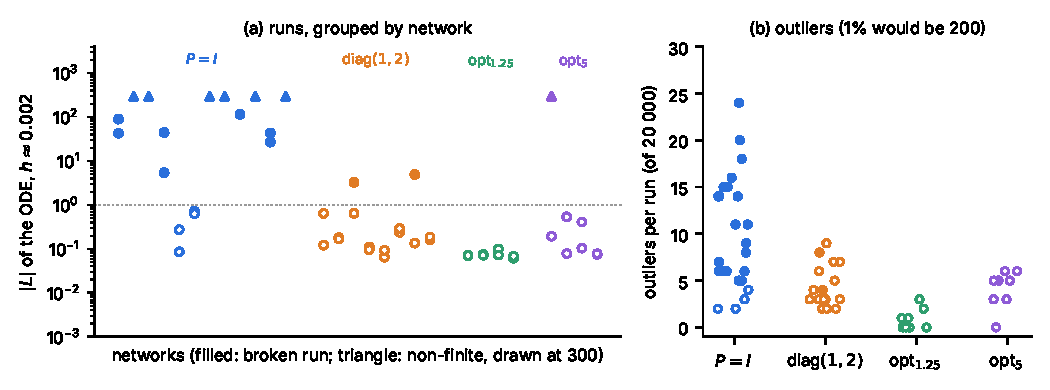
\includegraphics[width=\textwidth]{figures/fig2_ode}
\caption{Probability-flow ODE \Sc{} with learned scores, $h\approx0.002$.
(a)~$|L|$ of every run, grouped by network (two seeds per network); filled: broken runs; triangles: non-finite runs, drawn at 300.
Dotted: $|L|=1$.
(b)~Outliers per run, out of $20\,000$; filled: broken runs.}
\label{fig:ode}
\end{figure*}
